\subsection{Why source objective separation is not a validated switching rule}
\label{sec:source-target-not-predictor}
A limitation of objective-alignment scores is that they can appear
actionable without having been tested as prospective predictors of an
unseen person's gain. We therefore performed a clearly labelled
\emph{post-outcome descriptive} check using the \emph{original}
independently frozen Shin2017A score artifact. For each of the 29
outer participant folds, we read the original source-person AUC
path, its covariance-NLL path and the \emph{unchanged} held-person
model comparisons. Each source path was produced without the
held person's labels or feature statistics. The outer training pools
overlap heavily, so the 29 pairs do not constitute independent
source-to-deployment experiments.

The chosen discrimination criterion exceeded the AUC of the
source covariance-optimal candidate in all 29 folds, by
0.02605 source macro-AUC on average; it incurred a mean
source covariance-NLL cost of 0.72799 in the corresponding
per-dimension units. Both source-selected and
covariance-selected values came from the original same-grid
source validation. Yet that within-source separation was
\emph{not} proportional to the held-person benefit
(Fig.~\ref{fig:shin-posthoc-source-target}): the post-outcome
rank association of source AUC advantage with the target
AUC contrast was descriptively negative (Spearman
$\rho=-0.543$). A conventional independent-pairs
$p$-value is invalid here because most folds reuse the same
source participants. We make no general predictive or causal
claim from this exploratory association, and specify no
decision threshold using target outcomes.

\begin{table}[tb]
\centering
\small
\caption{Post-outcome robustness of the \emph{separately frozen}
Shin2017A (29 people). All contrasts refer to the same
original participant score family. Monte Carlo checks were
repeated for integrity only; the original family-adjusted
$p$-values remain the primary inference.}
\label{tab:shin-posthoc-robust}
\begin{tabular}{lcc}
\toprule
Post-outcome summary & vs Cov-NLL & vs Ledoit--Wolf\\
\midrule
Mean $\Delta$AUC (original) & +0.02222 & +0.04866\\
Median $\Delta$AUC & +0.01778 & +0.04667\\
10\% trimmed mean & +0.02062 & +0.04507\\
Minimum 1-person-deletion mean & +0.01750 & +0.04254\\
Maximum 1-person-deletion mean & +0.02623 & +0.05278\\
People harmed by $>0.02$ AUC & 5/29 & 3/29\\
\bottomrule
\end{tabular}
\end{table}

Every one-person omission retained a positive cohort mean,
but even a bootstrap or deletion check conditional on these
overlapping source fits does not establish a participant-safe
adaptive policy. In particular, the harmed fraction against
covariance-NLL was 17.2\% (5/29), with an exploratory Wilson
95\% interval of approximately 7.6--34.5\%;
the comparable Ledoit--Wolf fraction was 10.3\% (3/29).
Those intervals do not account for variation across new
EEG acquisition sites or independently retrained source pools.
They express uncertainty under a much narrower sampling
model, and are not medical safety intervals.

\begin{figure}[tb]
\centering
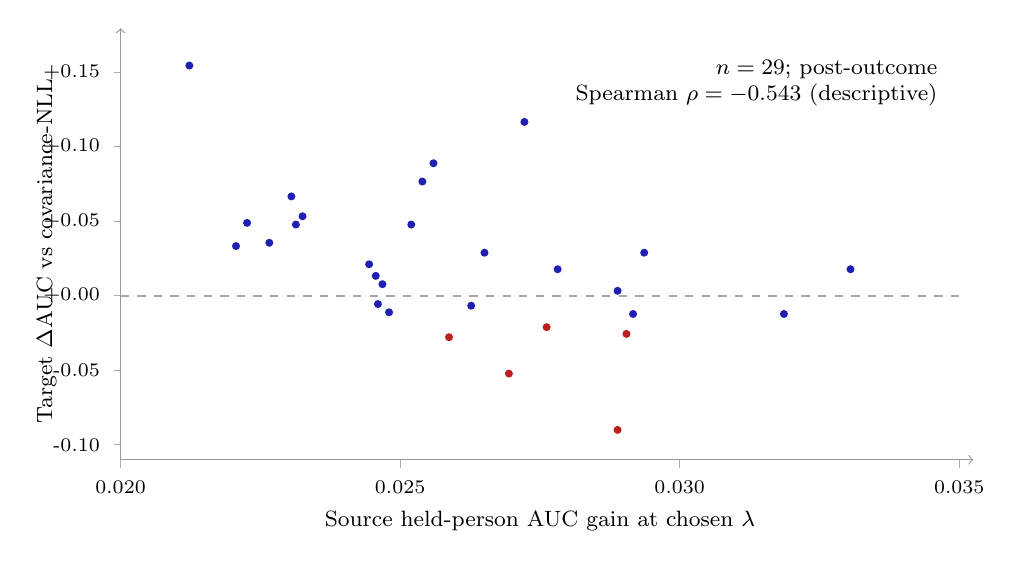
\begin{tikzpicture}[x=1cm,y=1cm]
\draw[->,gray!80] (1.450,1.000) -- (12.280,1.000);
\draw[->,gray!80] (1.450,1.000) -- (1.450,6.480);
\draw[dashed,gray!70,line width=.55pt] (1.450,3.082) -- (12.100,3.082);
\draw[gray!65] (1.360,1.189) -- (1.450,1.189);
\node[anchor=east,font=\scriptsize] at (1.310,1.189) {-0.10};
\draw[gray!65] (1.360,2.136) -- (1.450,2.136);
\node[anchor=east,font=\scriptsize] at (1.310,2.136) {-0.05};
\draw[gray!65] (1.360,3.082) -- (1.450,3.082);
\node[anchor=east,font=\scriptsize] at (1.310,3.082) {+0.00};
\draw[gray!65] (1.360,4.029) -- (1.450,4.029);
\node[anchor=east,font=\scriptsize] at (1.310,4.029) {+0.05};
\draw[gray!65] (1.360,4.975) -- (1.450,4.975);
\node[anchor=east,font=\scriptsize] at (1.310,4.975) {+0.10};
\draw[gray!65] (1.360,5.921) -- (1.450,5.921);
\node[anchor=east,font=\scriptsize] at (1.310,5.921) {+0.15};
\draw[gray!65] (1.450,1.000) -- (1.450,0.900);
\node[anchor=north,font=\scriptsize] at (1.450,0.850) {0.020};
\draw[gray!65] (5.000,1.000) -- (5.000,0.900);
\node[anchor=north,font=\scriptsize] at (5.000,0.850) {0.025};
\draw[gray!65] (8.550,1.000) -- (8.550,0.900);
\node[anchor=north,font=\scriptsize] at (8.550,0.850) {0.030};
\draw[gray!65] (12.100,1.000) -- (12.100,0.900);
\node[anchor=north,font=\scriptsize] at (12.100,0.850) {0.035};
\node[font=\footnotesize,align=center] at (6.775,0.220) {Source held-person AUC gain at chosen $\lambda$};
\node[rotate=90,font=\footnotesize] at (0.510,3.650) {Target $\Delta$AUC vs covariance-NLL};
\fill[blue!65!black,opacity=.88] (10.719,3.419) circle (1.45pt);
\fill[blue!65!black,opacity=.88] (5.423,4.765) circle (1.45pt);
\fill[blue!65!black,opacity=.88] (3.056,4.008) circle (1.45pt);
\fill[blue!65!black,opacity=.88] (3.619,4.344) circle (1.45pt);
\fill[blue!65!black,opacity=.88] (3.676,3.987) circle (1.45pt);
\fill[blue!65!black,opacity=.88] (3.338,3.755) circle (1.45pt);
\fill[red!70!black,opacity=.88] (6.381,2.094) circle (1.45pt);
\fill[blue!65!black,opacity=.88] (2.323,6.006) circle (1.45pt);
\fill[blue!65!black,opacity=.88] (7.761,3.145) circle (1.45pt);
\fill[blue!65!black,opacity=.88] (4.859,2.872) circle (1.45pt);
\fill[blue!65!black,opacity=.88] (8.099,3.629) circle (1.45pt);
\fill[red!70!black,opacity=.88] (7.874,2.598) circle (1.45pt);
\fill[red!70!black,opacity=.88] (7.761,1.379) circle (1.45pt);
\fill[blue!65!black,opacity=.88] (9.874,2.851) circle (1.45pt);
\fill[blue!65!black,opacity=.88] (5.141,3.987) circle (1.45pt);
\fill[blue!65!black,opacity=.88] (6.071,3.629) circle (1.45pt);
\fill[blue!65!black,opacity=.88] (4.718,2.977) circle (1.45pt);
\fill[blue!65!black,opacity=.88] (5.902,2.956) circle (1.45pt);
\fill[blue!65!black,opacity=.88] (4.690,3.335) circle (1.45pt);
\fill[blue!65!black,opacity=.88] (2.915,3.713) circle (1.45pt);
\fill[red!70!black,opacity=.88] (5.620,2.556) circle (1.45pt);
\fill[blue!65!black,opacity=.88] (4.606,3.482) circle (1.45pt);
\fill[blue!65!black,opacity=.88] (4.775,3.229) circle (1.45pt);
\fill[blue!65!black,opacity=.88] (7.958,2.851) circle (1.45pt);
\fill[blue!65!black,opacity=.88] (7.000,3.419) circle (1.45pt);
\fill[blue!65!black,opacity=.88] (3.760,4.092) circle (1.45pt);
\fill[blue!65!black,opacity=.88] (6.578,5.290) circle (1.45pt);
\fill[blue!65!black,opacity=.88] (5.282,4.533) circle (1.45pt);
\fill[red!70!black,opacity=.88] (6.860,2.683) circle (1.45pt);
\node[anchor=north east,font=\footnotesize,fill=white,inner sep=2pt,align=right] at (11.900,6.150) {$n=29$; post-outcome\\Spearman $\rho=-0.543$ (descriptive)};
\end{tikzpicture}
\caption{Exploratory, non-predictive sensitivity analysis on the 29 original Shin2017A frozen folds. Source-only held-source AUC advantage is compared against realised held-person AUC benefit. Red points denote participants harmed by more than 0.02 AUC. Training-source pools strongly overlap across outer folds, so these points cannot support an independent-samples correlation test or a prospective switching threshold. These observations were analysed after the original outcome release.}
\label{fig:shin-posthoc-source-target}
\end{figure}

